\chapter{Second phase formation in Bayer alumina}

\section{Introduction}
It is reported in the literature that dopants and impurities such as MgO, CaO, and Na$_{2}$O can form second phases such as spinel, calcium hexaluminate, and $\beta$-Al$_{2}$O$_{3}$, respectively, if their concentration is high enough. For Bayer aluminas $\beta$-Al$_{2}$O$_{3}$ is of particular interest because Na$_{2}$O impurities are characteristic to Bayer alumina and small amounts of a few hundred ppm can be sufficient to form $\beta$-Al$_{2}$O$_{3}$. Rankin and Merwin \cite{Rankin1916} were the first to observe the formation of a new alumina phase in the high Al$_{2}$O$_{3}$ region in the system CaO-Al$_{2}$O$_{3}$-MgO. They believed it was an allotropic modification of Al$_{2}$O$_{3}$, and named it $\beta$-Al$_{2}$O$_{3}$. However, later work clarified that there is a relation between the alkali content in the Al$_{2}$O$_{3}$ and the formation of $\beta$-Al$_{2}$O$_{3}$ \cite{Stillwell1926}, and that $\beta$-Al$_{2}$O$_{3}$ is an alkali aluminate, rather than an allotropic form of Al$_{2}$O$_{3}$ \cite{Vries1969}. Ridgway et al. \cite{Ridgway1936} reported that the Na$_{2}$O content in Bayer process alumina can be high enough for the formation of $\beta$-Al$_{2}$O$_{3}$, and that $\beta$-Al$_{2}$O$_{3}$ forms in "dry ore process" Al$_{2}$O$_{3}$ (with unspecified low concentrations of Na$_{2}$O) only when Na$_{2}$O or K$_{2}$O is added. Four types of $\beta$-Al$_{2}$O$_{3}$ exist; two of them, $\beta$-Al$_{2}$O$_{3}$ (Na$_{2}$O*11Al$_{2}$O$_{3}$) and $\beta$''-Al2O3 (Na2O.5Al2O3), form in the binary system Na$_{2}$O-Al$_{2}$O$_{3}$, and can incorporate MgO. The other two beta aluminas, $\beta$'''-Al$_{2}$O$_{3}$ and $\beta$''''-Al$_{2}$O$_{3}$ are found in the ternary system Na$_{2}$O-Al$_{2}$O$_{3}$-MgO \cite{Stevens1984}. For completeness it should be mentioned that the existence of a $\beta$'-Al$_{2}$O$_{3}$ (Na$_{2}$O*7Al$_{2}$O$_{3}$) has been reported as well, but subsequent literature is in agreement that $\beta$'-Al$_{2}$O$_{3}$ is actually $\beta$-Al$_{2}$O$_{3}$ with excess Na$_{2}$O \cite{Stevens1984}.

The formation and stability of $\beta$-Al$_{2}$O$_{3}$ has been extensively studied in the literature because its excellent ion conductivity makes it suitable for applications as a solid electrolyte; especially for use in batteries. Most reported preparation routs involve sodium carbonate and alumina \cite{Vries1969,Kummer1972,Ray1975}. Heating mixtures of alumina and sodium carbonate to 1100$^{\circ}$C leads to the formation of $\beta$''-Al$_{2}$O$_{3}$, which decomposes to $\beta$-Al$_{2}$O$_{3}$ and NaAlO$_{2}$ at temperatures >1500$^{\circ}$C. The equilibrium vapor pressure of Na$_{2}$O over $\beta$-Al$_{2}$O$_{3}$ has been reported to be "appreciable" at temperatures >1400$^{\circ}$C \cite{Kummer1972}, where $\beta$-Al$_{2}$O$_{3}$ can decompose to $\alpha$-Al$_{2}$O$_{3}$ by volatilization of Na$_{2}$O. However, soda loss has been reported to occur at lower temperatures as well, e.g. 6.4 wt\% of soda loss was reported by de Vries and Roth \cite{Vries1969} when they prepared $\beta$''-alumina samples and heated it for 4 h at 1100 $^{\circ}$C. On the other hand, Gallup \cite{Gallup1935} investigated the stability of $\beta$-Al$_{2}$O$_{3}$ at high temperatures and under different atmospheres and he reported that $\beta$-Al$_{2}$O$_{3}$ can convert to $\alpha$-Al$_{2}$O$_{3}$ at temperatures as low as 1300$^{\circ}$C in hydrogen or vacuum atmosphere, but in air no conversion was observed for heating as long as 1 h at 1500$^{\circ}$C. Full conversion was observed when the material was heated for 10 min at 1600$^{\circ}$C.

Even though the conditions for the formation of $\beta$-Al$_{2}$O$_{3}$ in $\alpha$-Al$_{2}$O$_{3}$ ceramics are of great importance, especially because the Na$_{2}$O content in Bayer process Al$_{2}$O$_{3}$ is sufficient for the formation of $\beta$-Al$_{2}$O$_{3}$, it is barely studied in literature. Duncan and Creyke \cite{Duncan1969a} investigated the formation and stability of $\beta$-Al$_{2}$O$_{3}$ in $\alpha$-Al$_{2}$O$_{3}$ ceramics and used two commercial alumina powders with impurities of 0.038 wt\% SiO$_{2}$, 0.006 wt\% MgO and 0.061 ppm Na$_{2}$O, and 0.04 wt\% SiO$_{2}$, 0.2 wt\% MgO and 0.04 wt\% Na$_{2}$O, respectively. They reported that $\beta$-Al$_{2}$O$_{3}$ can form at Na$_{2}$O concentrations as low as 300 ppm if a small amount of MgO is present. They estimated the amount of $\beta$-Al$_{2}$O$_{3}$ by measuring the dielectric loss of the sample, since $\beta$-Al$_{2}$O$_{3}$ was observed to increase the dielectric loss of $\alpha$-Al$_{2}$O$_{3}$ samples. An increase in amount of $\beta$-Al$_{2}$O$_{3}$ was observed with increasing Na$_{2}$O, but also with increasing MgO additions, and it was shown by electron-probe microanalysis that there is a higher concentration of Na$_{2}$O and MgO in the $\beta$-Al$_{2}$O$_{3}$ grains. They state that samples, in which $\beta$-Al$_{2}$O$_{3}$ forms, show no formation of spinel \cite{Duncan1969a} and furthermore they determined that $\beta$-Al$_{2}$O$_{3}$ in $\alpha$-Al$_{2}$O$_{3}$ is stable to up to 1650 $^{\circ}$C in stagnant air. In a flowing air stream, however, decomposition to $\alpha$-Al$_{2}$O$_{3}$ takes place, even in the center of the sample and the decomposition is facilitated by open porosity and higher temperatures, whereas a high degree of compaction of the powder, e.g. a high green density, impedes the decomposition. Small amounts of other oxides (e.g. SiO$_{2}$, MgO, ZrO$_{2}$) are reported to facilitate the decomposition process due to an easier diffusion path through the grain boundaries. The work by Duncan and Creyke focuses on the decomposition and while some literature reports indicate under what conditions $\beta$-Al$_{2}$O$_{3}$ may form \cite{Duncan1969a}, there is no systematic study on the formation of $\beta$-Al$_{2}$O$_{3}$ as function of powder chemistry, at what sintering stage $\beta$-Al$_{2}$O$_{3}$ forms and what possible formation mechanisms are. Goal of this work is to identify the stages and mechanisms of $\beta$-Al$_{2}$O$_{3}$ formation in $\alpha$-Al$_{2}$O$_{3}$.


\section{Experimental}

The samples fabricated for the investigations in Chapters 2 and 3 were used to investigate the formation of $\beta$-Al$_{2}$O$_{3}$ in $\alpha$-Al$_{2}$O$_{3}$. To investigate the influence of MgO concentration on the formation of $\beta$-Al$_{2}$O$_{3}$ the MgO-free powder used in Chaper 2 was also doped with up to 1000 ppm MgO using magnesium nitrate hexahydrate (Mg(NO$_{3}$)$_{2}$*6H$_{2}$O, 99.97\%, Alfa Aesar, Ward Hill, MA, USA). The alumina powder was dispersed in aqueous magnesium nitrate solution and stirred on a magnetic stir plate for 5 h at room temperature, and then held at 80 $^{\circ}$C for 24 h until the mixture was too viscous to stir. The mixture was then placed in a drying oven at 100 $^{\circ}$C for 24 h to thoroughly dry the powder. Additionally, an ultra-high purity powder (AKP-50, Sumitomo Chemical Co. Ltd., Tokyo, Japan) was doped with up to 2000 ppm Na$_{2}$O, 500 ppm SiO$_{2}$, and 500 ppm MgO and used to dry press samples. The intrinsic impurities in the ultra high purity powder are 11 ppm SiO$_{2}$, 4 ppm Fe2O3, 2 ppm Na$_{2}$O, 2 ppm MgO, and 1 ppm Cu. The doping and sample preparation procedure is described in detail in chapters 2 and 3.

\section{Results}

Initially the detection of $\beta$-Al$_{2}$O$_{3}$ in an $\alpha$-Al$_{2}$O$_{3}$ matrix was investigated. Figure \ref{Ch5-figure:Figure1}a-c shows SEM micrographs of $\beta$-Al$_{2}$O$_{3}$ grains in a sample with 529 ppm Na$_{2}$O, 103 ppm SiO$_{2}$, and 380 ppm MgO sintered at 1525$^{\circ}$C for 3 h. It can be seen that in unetched samples $\beta$-Al$_{2}$O$_{3}$ grains can hardly be observed in images obtained from secondary electrons (Figure \ref{Ch5-figure:Figure1}a). Figure \ref{Ch5-figure:Figure1}b shows an SEM image of the same area of the sample as Figure \ref{Ch5-figure:Figure1}a obtained from the backscattered electrons and a stronger contrast between the $\beta$-Al$_{2}$O$_{3}$ grains and the surrounding $\alpha$-Al$_{2}$O$_{3}$ matrix can be seen, which is due to the higher sensitivity of backscattered electrons to density. $\beta$-Al$_{2}$O$_{3}$ grains appear darker due to the lower density (3.31 g/cm$^{3}$) compared to $\alpha$-Al$_{2}$O$_{3}$ (3.986 g/cm$^{3}$). Figure \ref{Ch5-figure:Figure1}c shows a $\beta$-Al$_{2}$O$_{3}$ grain after thermal etching at 1425$^{\circ}$C for 40 min and it can be seen that the $\beta$-Al$_{2}$O$_{3}$ grain has evaporated during thermal etching, leaving a platelet shaped hole in the etched microstructure. It is interesting to note that samples with low Na$_{2}$O concentrations such as 29 ppm form $\beta$-Al$_{2}$O$_{3}$ grains that do not evaporate during thermal etching, as seen in Figure \ref{Ch5-figure:Figure1}d. SEM micrographs obtained from backscattered electrons were used to detect $\beta$-Al$_{2}$O$_{3}$ grains for the following investigations.

\subsection{Influence of MgO on the formation of $\beta$-Al$_{2}$O$_{3}$}

Figure \ref{Ch5-figure:Figure2}a shows the influence of MgO concentration on the number of $\beta$-Al$_{2}$O$_{3}$ grains after sintering at 1525$^{\circ}$C for 3 h. It can be seen that for a MgO concentration of 2 ppm no $\beta$-Al$_{2}$O$_{3}$ was observed, and with increasing the MgO concentration the number of $\beta$-Al$_{2}$O$_{3}$ grains that form increases up to 502 ppm MgO, but does not increase further when the MgO concentration is increased to 1002 ppm. This shows that MgO assists the formation of $\beta$-Al$_{2}$O$_{3}$. The influence of Na2O concentration on the number of $\beta$-Al$_{2}$O$_{3}$ grains in MgO-free Bayer alumina after sintering at 1525$^{\circ}$C for 3 h is shown in Figure \ref{Ch5-figure:Figure2}b. It can be seen that only a small number of $\beta$-Al$_{2}$O$_{3}$ grains form for concentrations $\leq$ 529 ppm Na2O, but for higher concentrations, such as 1029 ppm, the number of $\beta$-Al$_{2}$O$_{3}$ grains increases significantly. Since commercial Bayer aluminas are typically doped with MgO, the following investigations are focused on Bayer alumina powder that was doped with 380 ppm MgO.

\subsection{MgO-doped Bayer alumina}
\subsubsection{Number frequency of $\beta$-Al$_{2}$O$_{3}$ grains}

Figure \ref{Ch5-figure:Figure3} shows the influence of the Na$_{2}$O and SiO$_{2}$ concentration on the number density of $\beta$-Al$_{2}$O$_{3}$ grains in Bayer alumina powder doped with 380 ppm MgO. It can be seen that the number density of $\beta$-Al$_{2}$O$_{3}$ grains increases with increasing Na$_{2}$O concentration (Figure \ref{Ch5-figure:Figure3}a), but decreases as a function of SiO$_{2}$ concentration in samples with different Na$_{2}$O concentrations (Figure \ref{Ch5-figure:Figure3}b). This indicates that the Na$_{2}$O/SiO$_{2}$ ratio determines the number density of $\beta$-Al$_{2}$O$_{3}$ grains. Figure \ref{Ch5-figure:Figure3}c shows the number density of $\beta$-Al$_{2}$O$_{3}$ grains as a function of the Na$_{2}$O/SiO$_{2}$ ratio, and it can be seen that the number density of $\beta$-Al$_{2}$O$_{3}$ grains increases linearly with increasing Na$_{2}$O/SiO$_{2}$ ratio. 

The kinetics of $\beta$-Al$_{2}$O$_{3}$ formation at 1525$^{\circ}$C for different powder chemistries (MgO-doped Bayer alumina) is shown in Figure \ref{Ch5-figure:Figure4}. Most $\beta$-Al$_{2}$O$_{3}$ grains forms within the first hour at 1525$^{\circ}$C, and after that the number density of $\beta$-Al$_{2}$O$_{3}$ grains does not change for all chemistries. In contrast, for samples prepared from ultra high purity powder (AKP-50) the amount of $\beta$-Al$_{2}$O$_{3}$ that forms during sintering in the temperature range from 1450$^{\circ}$C to 1600$^{\circ}$C for up to 8 h does not change, regardless of the Na$_{2}$O, MgO, or SiO$_{2}$ concentrations. However, in the ultra-high purity powder it was observed that increasing the Na$_{2}$O and MgO concentrations increases the number of $\beta$-Al$_{2}$O$_{3}$ grains in the microstructures, and increasing the SiO$_{2}$ concentration decreases the number of $\beta$-Al$_{2}$O$_{3}$ grains in the microstructures, similar to the Bayer alumina powder.

\subsubsection{Size of $\beta$-Al$_{2}$O$_{3}$ grains}
Figure \ref{Ch5-figure:Figure5} shows micrographs of samples with different powder chemistries with up to 1000 ppm MgO, Na$_{2}$O, and SiO$_{2}$ after sintering at 1525$^{\circ}$C for 3 h. It can be seen that the size of the $\beta$-Al$_{2}$O$_{3}$ grains changes as a function of powder chemistry. Samples with 1000 ppm MgO, 1000 ppm SiO$_{2}$, and 29 ppm Na$_{2}$O form 30-40 $\mu$m long $\beta$-Al$_{2}$O$_{3}$ grains (Figure \ref{Ch5-figure:Figure5}a). The $\beta$-Al$_{2}$O$_{3}$ grains that form in samples with 2 ppm MgO, 1000 ppm SiO$_{2}$, and 1000 ppm Na$_{2}$O are 10-20 $\mu$m long (Figure \ref{Ch5-figure:Figure5}b), and the $\beta$-Al$_{2}$O$_{3}$ grains in samples with 1000 ppm MgO, 1000 ppm SiO$_{2}$, and 1000 ppm Na$_{2}$O are 4-10 $\mu$m long (Figure \ref{Ch5-figure:Figure5}c). Note that no $\beta$-Al$_{2}$O$_{3}$ was observed in samples with 29 ppm Na$_{2}$O and 2 ppm MgO, regardless of the SiO$_{2}$ concentration.

Micrographs of MgO-doped (380 ppm) Bayer alumina with Na$_{2}$O concentrations of up to 1060 ppm Na$_{2}$O sintered at 1525$^{\circ}$C for 3 h are shown in Figure \ref{Ch5-figure:Figure6}. The $\beta$-Al$_{2}$O$_{3}$ grains are 3-13 $\mu$m long for samples with 185 ppm Na$_{2}$O and 4-10 $\mu$m for samples with 560 ppm Na$_{2}$O, and if the Na$_{2}$O concentration is increased to 1060 ppm the $\beta$-Al$_{2}$O$_{3}$ grains are significantly smaller (2-7 $\mu$m).

Micrographs of samples with 185/182 ppm Na$_{2}$O/SiO$_{2}$ and 560/182 ppm Na$_{2}$O/SiO$_{2}$ after sintering at 1525$^{\circ}$C for 3 h are shown in Figure \ref{Ch5-figure:Figure7}. The Na$_{2}$O concentrations in those samples are the same as in the samples in Figure \ref{Ch5-figure:Figure6}a and b, respectively. However, the samples in Figure \ref{Ch5-figure:Figure7} contain 100 ppm more SiO$_{2}$. It can be seen that higher SiO$_{2}$ concentrations lead to larger $\beta$-Al$_{2}$O$_{3}$ grains compared to samples with lower SiO$_{2}$ concentrations.

Figure \ref{Ch5-figure:Figure8} shows micrographs of MgO-doped (380 ppm) Bayer alumina samples with 560 ppm Na$_{2}$O and 82 ppm SiO$_{2}$ after heating for 0 h, 1 h, and 8 h. It can be seen that the size of the $\beta$-Al$_{2}$O$_{3}$ grains does not change as a function of sintering time. However, as shown in Figure \ref{Ch5-figure:Figure4}, the number of the $\beta$-Al$_{2}$O$_{3}$ grains increases with increasing sintering time.

Figure \ref{Ch5-figure:Figure9} show the XRD pattern of a polished sample with 1060 ppm Na$_{2}$O, 582 ppm SiO$_{2}$ and 380 ppm MgO after sintering at 1525$^{\circ}$C for 5 h. The pattern shows that there is a small amount of $\beta$-Al$_{2}$O$_{3}$ present with P6$_{3}$/mmc crystal structure, which can be assigned to $\beta$-Al$_{2}$O$_{3}$. The estimated amount of $\beta$-Al$_{2}$O$_{3}$ from the XRD pattern is 0.6 wt.\%. EDS reveals that the $\beta$-Al$_{2}$O$_{3}$ grains contain higher concentrations of MgO and Na$_{2}$O compared to the surrounding matrix.

Since the type of $\beta$-Al$_{2}$O$_{3}$ that forms is known a theoretical volume fraction of $\beta$-Al$_{2}$O$_{3}$ can be estimated based on the chemical formula of $\beta$-Al$_{2}$O$_{3}$ (Na$_{2}$O*11Al$_{2}$O$_{3}$) and the amount of Na$_{2}$O in the samples, as seen in Table \ref{Ch5-table:table1}. The size of the $\beta$-Al$_{2}$O$_{3}$ grains was measured from the SEM images (length and thickness) and an area fraction was estimated. The estimated area fraction is assumed to be equal to the volume fraction of $\beta$-Al$_{2}$O$_{3}$ in the sample. It can be seen that the theoretically estimated amount of $\beta$-Al$_{2}$O$_{3}$ that can form based on the amount of Na$_{2}$O in the samples is higher than the observed amount of $\beta$-Al$_{2}$O$_{3}$ in the samples. A possible explanation is that some amount of Na$_{2}$O might volatize during sintering, as shown in Chapter 3. Taking into account that 35\% of the Na$_{2}$O might volatize during heating (Figure \ref{Ch3-figure:Figure12} Chapter 3), the expected amount of $\beta$-Al$_{2}$O$_{3}$ in the samples is close to the observed amount of $\beta$-Al$_{2}$O$_{3}$, as seen in Table \ref{Ch5-table:table1}.

\subsection{Interpretation and mechanisms of formation}

TEM and EDS analysis showed that insoluble impurities and dopants such as Na$_{2}$O, MgO, CaO and SiO$_{2}$ segregate to the grain boundaries. In general it can be assumed that second phases can form when the solubility of impurities and dopants in the bulk and in the grain boundaries is exceeded. In the MgO-free powder it can be seen that no second phase forms for Na$_{2}$O concentrations of 29 ppm, and only a very small amount of $\beta$-Al$_{2}$O$_{3}$ forms in samples with 529 ppm Na$_{2}$O. When the Na$_{2}$O concentration is increased to 1029 ppm the amount of $\beta$-Al$_{2}$O$_{3}$ that froms increases drastically (Figure \ref{Ch5-figure:Figure2}b). This indicates that the solubility of Na$_{2}$O in the grains and grain boundaries in the MgO-free alumina is $\sim$500 ppm Na$_{2}$O (note the presence of 103 ppm SiO$_{2}$ in the MgO-free powder). For higher Na$_{2}$O concentrations the grain boundaries supersaturate during sintering and $\beta$-Al$_{2}$O$_{3}$ forms. If the SiO$_{2}$ concentration in MgO-free powder samples is increased no $\beta$-Al$_{2}$O$_{3}$ forms and we believe that SiO$_{2}$ significantly increases the Na$_{2}$O solubility in the grain boundaries by forming a liquid grain boundary phase. The argument that SiO$_{2}$ increases the solubility of Na$_{2}$O in the grain boundaries is further supported by the observation that a considerable number of $\beta$-Al$_{2}$O$_{3}$ grains form in the ultra high purity powder with 502 ppm Na$_{2}$O, 2 ppm MgO and 11 ppm SiO$_{2}$, as seen in Figure \ref{Ch5-figure:Figure10}, whereas almost no $\beta$-Al$_{2}$O$_{3}$ grains were observed in MgO-free Bayer alumina samples with 529 ppm Na$_{2}$O, 2 ppm MgO, and 103 ppm SiO$_{2}$. 

When the MgO concentration in Bayer alumina is increased $\beta$-Al$_{2}$O$_{3}$ forms at significantly lower Na$_{2}$O concentrations, e.g. at Na$_{2}$O concentrations as low as 29 ppm. The amount of $\beta$-Al$_{2}$O$_{3}$ that forms increases with increasing MgO concentration up to 502 ppm. We believe that this is because MgO removes SiO$_{2}$ from the grain boundaries during sintering, as explained earlier, and this mechanism significantly decreases the solubility of Na$_{2}$O in the grain boundaries, leading to the nucleation of $\beta$-Al$_{2}$O$_{3}$. 

If it is assumed that MgO and SiO$_{2}$ form the defect complex proposed earlier, and if it is assumed that MgO and SiO$_{2}$ go into solid solution at equal amounts and that all MgO is consumed by this process, MgO-doped powder samples (380 ppm MgO) with 82 and 182 ppm SiO$_{2}$ do not have any SiO$_{2}$ left in the grain boundaries. This reduction in the amount of SiO$_{2}$ in the grain boundaries reduces the solubility of Na$_{2}$O in the grain boundaries significantly, leading to the precipitation of $\beta$-Al$_{2}$O$_{3}$. Samples with 582 ppm SiO$_{2}$ have 202 ppm SiO$_{2}$ left in the grain boundaries after 380 ppm MgO and SiO$_{2}$ co-dissolve into the alumina lattice, and the solubility of Na$_{2}$O in the grain boundaries is still high enough so that only few $\beta$-Al$_{2}$O$_{3}$ grains in this sample, due to the presence of 202 ppm SiO$_{2}$. 

The process of SiO$_{2}$ and MgO co-dissolving into the alumina lattice and the formation of $\beta$-Al$_{2}$O$_{3}$ happens at the same time, between 0 and 3 h at 1525$^{\circ}$C, which supports the hypothesis that $\beta$-Al$_{2}$O$_{3}$ nucleates and grows as a result of supersaturation of the grain boundaries when MgO removes SiO$_{2}$ from the grain boundaries. However, samples with 560 ppm Na$_{2}$O and 82 ppm SiO$_{2}$ form more $\beta$-Al$_{2}$O$_{3}$ than samples with 560 ppm Na$_{2}$O and 182 ppm SiO$_{2}$, even though no SiO$_{2}$ should be in the grain boundaries for both samples. One reason could be that not all 380 ppm MgO and SiO$_{2}$ are consumed by this co-dissolution process, and a small amount SiO$_{2}$ might remain on the grain boundaries, which would increase the Na$_{2}$O solubility. 

Another possible explanation is that MgO has an additional effect on the formation of $\beta$-Al$_{2}$O$_{3}$ in $\alpha$-Al$_{2}$O$_{3}$. It has been reported that MgO supports the formation of $\beta$-Al$_{2}$O$_{3}$ in alumina, and samples with 560 ppm Na$_{2}$O and 82 ppm SiO$_{2}$ have 100 ppm more MgO left in the grain boundaries than samples with 560 ppm Na$_{2}$O and 182 ppm SiO$_{2}$. Since EDS shows that MgO is in the $\beta$-Al$_{2}$O$_{3}$ grains MgO might facilitate the formation of $\beta$-Al$_{2}$O$_{3}$. 

\section{Summary}



\newpage
\begin{table}[H]
	\caption{Estimated amount of $\beta$-Al$_{2}$O$_{3}$ in MgO-doped (380 ppm) Bayer alumina samples after 3 h at 1525$^{\circ}$C.}
	\centering
	\begin{tabular}{ | c | c | c | c | }
		\hline
		Concentration of  & \multicolumn{2}{l|}{Theoretical vol.\% of $\beta$-Al$_{2}$O$_{3}$} & Measured amount \\
		\cline{2-3}
		Na$_{2}$O in & No Na$_{2}$O & Assuming 35 \% of & of $\beta$-Al$_{2}$O$_{3}$\\
		the sample (ppm) & volatizes & of Na$_{2}$O volatizes & 3h 1525$^{\circ}$\\		
		\hline
		60 & 0.14 & 0.09 & 0.18\\
		\hline
		185 & 0.42 & 0.28 & 0.25\\
		\hline
		310 & 0.71 & 0.46 & 0.38\\
		\hline
		560 & 1.28 & 0.84 & 0.65\\
		\hline
		1060 & 2.42 & 1.58 & 0.49\\
		\hline
	\end{tabular}
	\label{Ch5-table:table1}
\end{table}
\clearpage
%%%

\newpage
%%%
\begin{figure}[H]
	\centering
	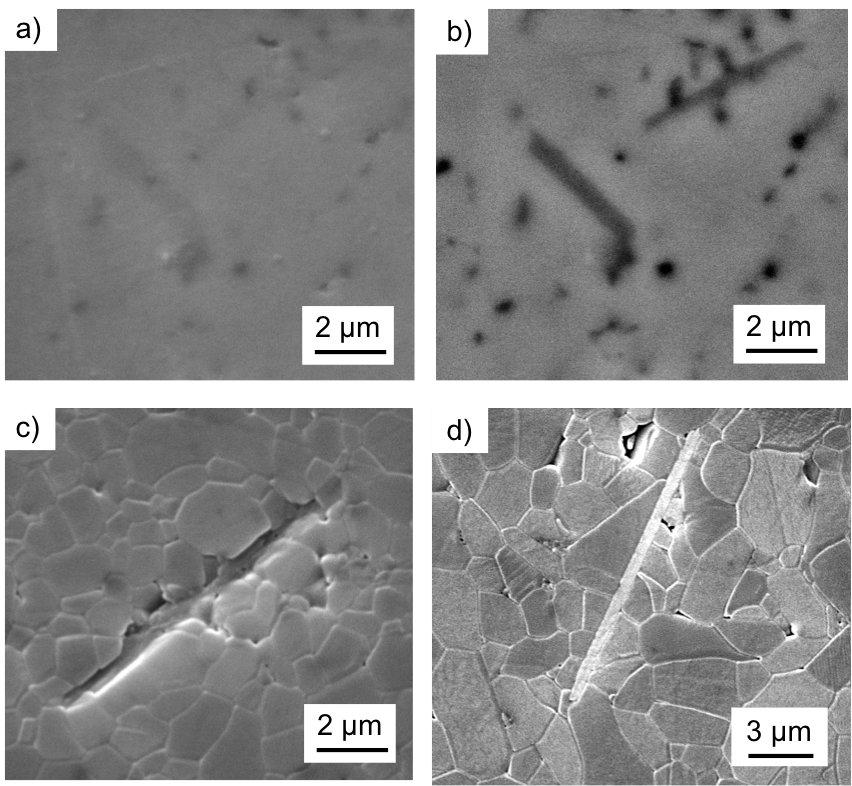
\includegraphics[width=\textwidth]{Chapter-5/Figures/Figure1.png}
	\caption{SEM micrographs of $\beta$-Al$_{2}$O$_{3}$ grains in a-c) Bayer alumina with 560 ppm Na$_{2}$O, 82 ppm SiO$_{2}$, and 380 ppm MgO after 3 h at 1525$^{\circ}$C and d) Bayer alumina with 29 ppm Na$_{2}$O, 103 ppm SiO$_{2}$, and 502 ppm MgO after 3 h at 1525$^{\circ}$C. The samples in a) and b) were not etched and the samples in c) and d) were etched. a), c), and d) were obtained using a secondary electron detector, and b) was obtained using a backscattered electron detector.}
	\label{Ch5-figure:Figure1}
\end{figure}
%%%

\newpage
%%%
\begin{figure}[H]
	\centering
	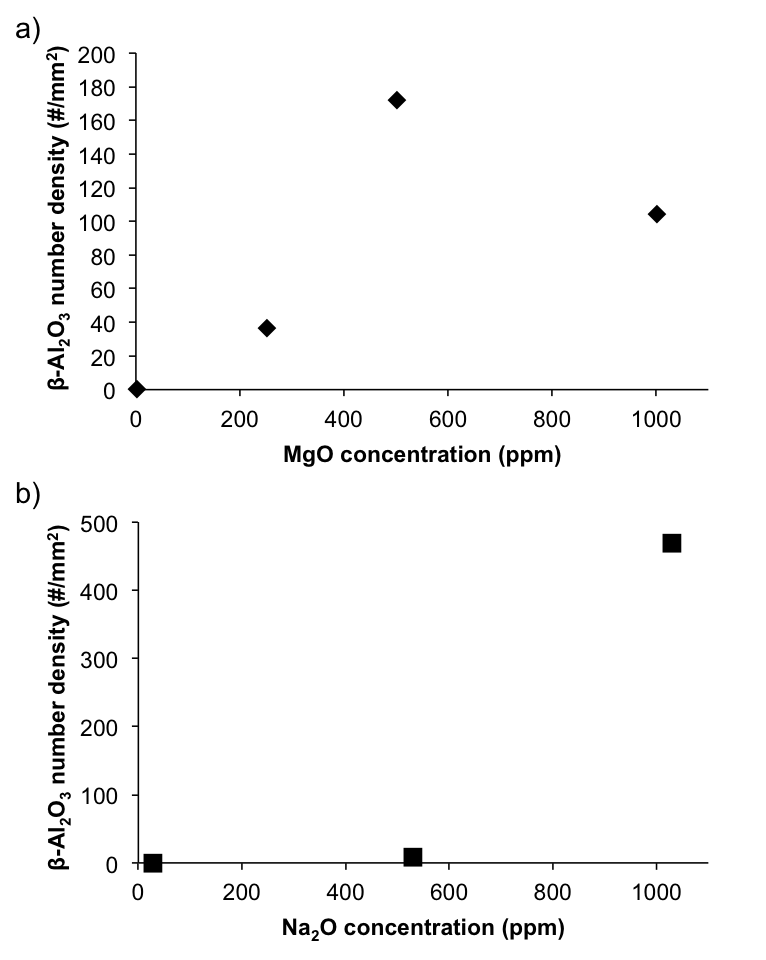
\includegraphics{Chapter-5/Figures/Figure2.png}
	\caption{Formation of $\beta$-Al$_{2}$O$_{3}$ in MgO-free powder samples as a function of a) MgO concentration and b) Na$_{2}$O concentration in samples after 3 h at 1525$^{\circ}$C.}
	\label{Ch5-figure:Figure2}
\end{figure}
%%%

\newpage
%%%
\begin{figure}[H]
	\centering
	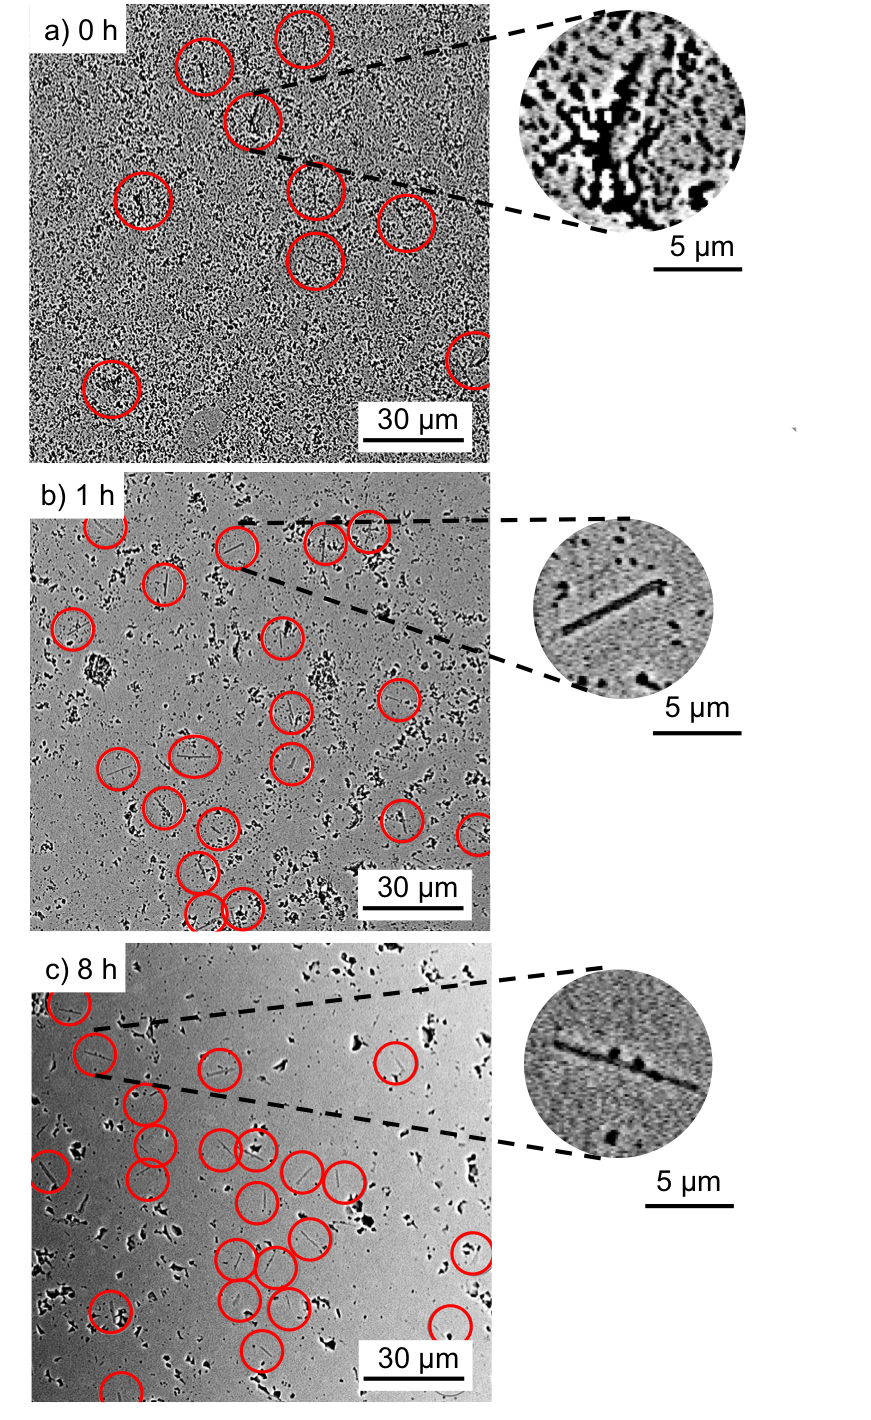
\includegraphics{Chapter-5/Figures/Figure3.png}
	\caption{Formation of $\beta$-Al$_{2}$O$_{3}$ a function of a) Na$_{2}$O concentration, b) SiO$_{2}$ concentration for different Na$_{2}$O concentrations, and c) of the Na$_{2}$O/SiO$_{2}$ ratio in MgO-doped (380 ppm) powder samples. In c) the black diamonds are samples with 82 ppm SiO$_{2}$ and the blue squares are samples with 182 and 582 ppm SiO$_{2}$.}
	\label{Ch5-figure:Figure3}
\end{figure}
%%%

\newpage
%%%
\begin{figure}[H]
	\centering
	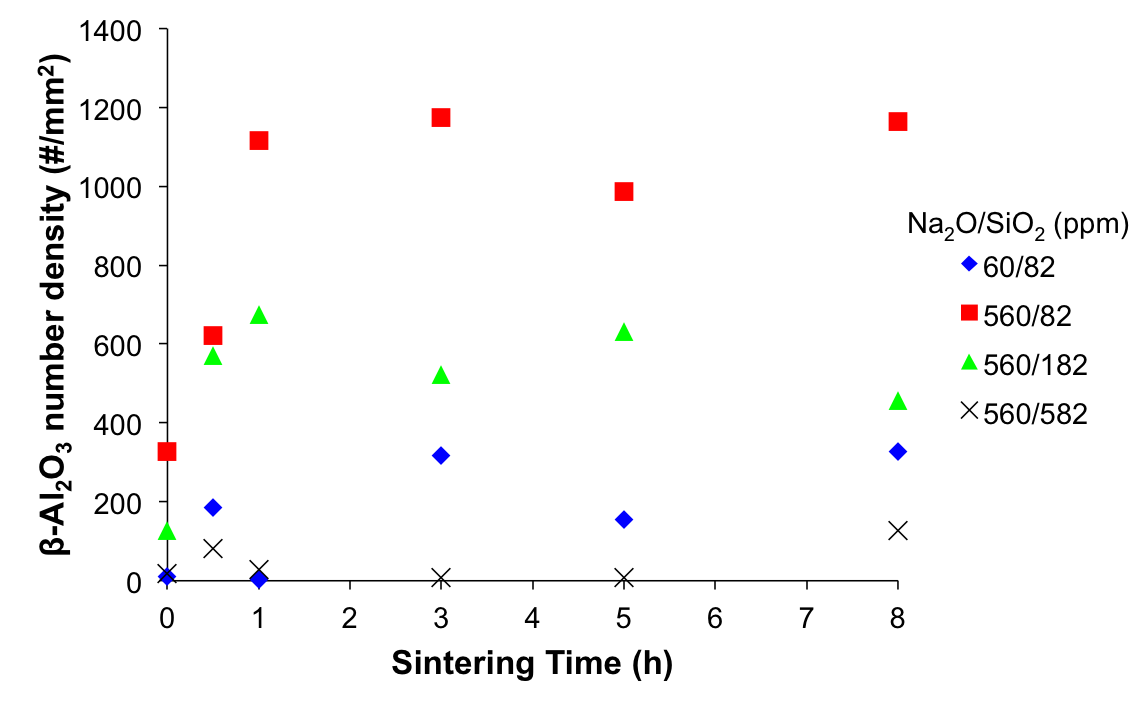
\includegraphics[width=\textwidth]{Chapter-5/Figures/Figure4.png}
	\caption{Kinetics of $\beta$-Al$_{2}$O$_{3}$ formation for different powder chemistries of MgO-doped powder samples (380 ppm MgO).}
	\label{Ch5-figure:Figure4}
\end{figure}
%%%

\newpage
%%%
\begin{figure}[H]
	\centering
	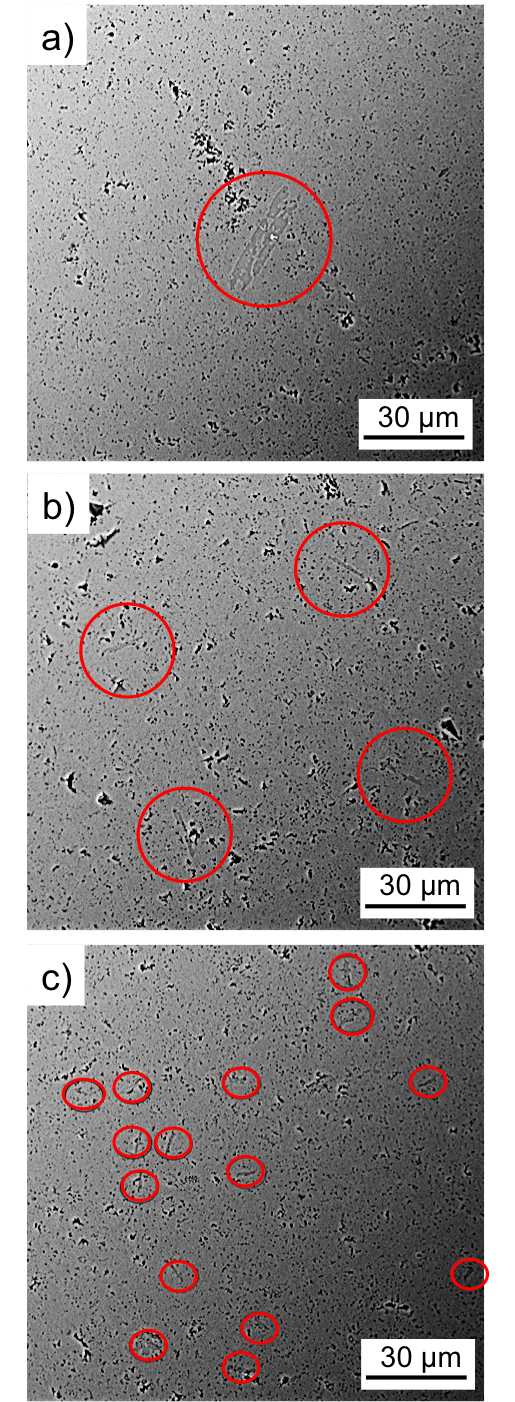
\includegraphics{Chapter-5/Figures/Figure5.png}
	\caption{Micrographs showing $\beta$-Al$_{2}$O$_{3}$ grains (red circles) in Bayer alumina samples with a) 1000 ppm MgO, 1000 ppm SiO$_{2}$, 29 ppm Na$_{2}$O, b) 2 ppm MgO, 1000 ppm SiO$_{2}$, 1000 ppm Na$_{2}$O, c) 1000 ppm MgO, 1000 ppm SiO$_{2}$, 1000 ppm Na$_{2}$O after 3 h at 1525$^{\circ}$C.}
	\label{Ch5-figure:Figure5}
\end{figure}
%%%

\newpage
%%%
\begin{figure}[H]
	\centering
	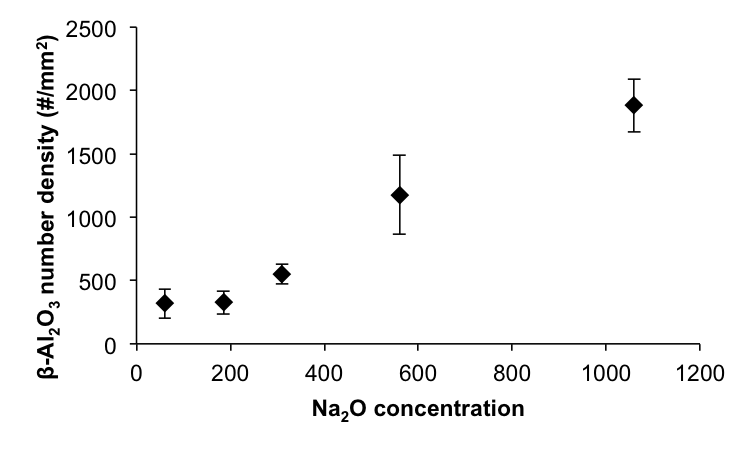
\includegraphics{Chapter-5/Figures/Figure6.png}
	\caption{Micrographs showing $\beta$-Al$_{2}$O$_{3}$ grains (red circles) in MgO-doped (380 ppm) Bayer alumina samples with 82 ppm SiO$_{2}$ and a) 185 ppm Na$_{2}$O, b) 560 ppm Na$_{2}$O, and c) 1060 ppm Na$_{2}$O after sintering at 1525$^{\circ}$C for 3 h.}
	\label{Ch5-figure:Figure6}
\end{figure}
%%%

\newpage
%%%
\begin{figure}[H]
	\centering
	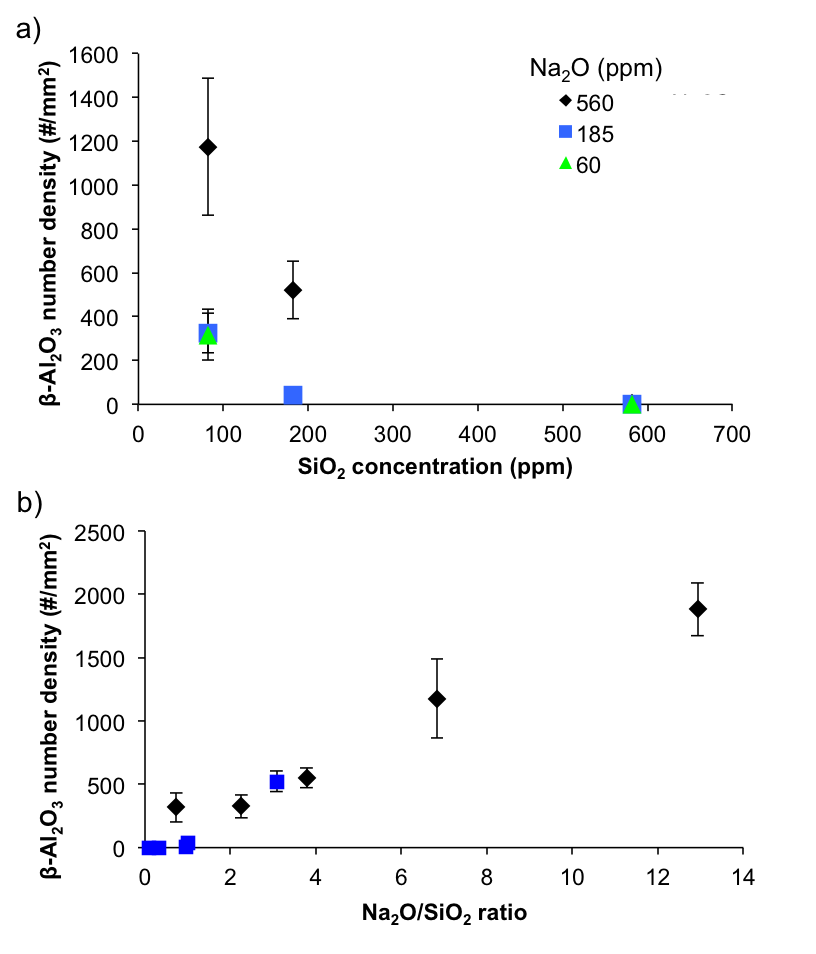
\includegraphics{Chapter-5/Figures/Figure7.png}
	\caption{Micrographs showing $\beta$-Al$_{2}$O$_{3}$ grains (red circles) in MgO-doped (380 ppm) Bayer alumina samples with a) 185/182 ppm Na$_{2}$O/SiO$_{2}$ and b) 560/182 ppm Na$_{2}$O/SiO$_{2}$ after sintering at 1525$^{\circ}$C for 3 h.}
	\label{Ch5-figure:Figure7}
\end{figure}
%%%

\newpage
%%%
\begin{figure}[H]
	\centering
	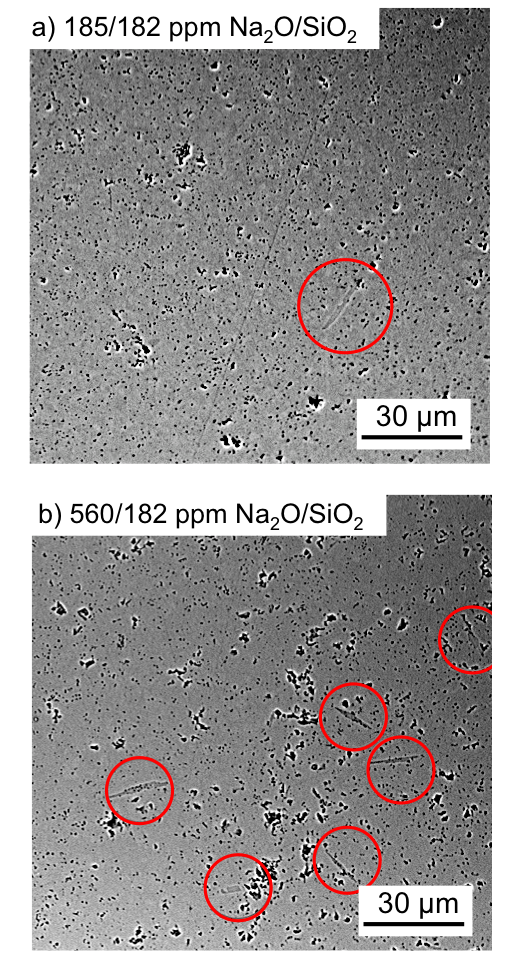
\includegraphics{Chapter-5/Figures/Figure8.png}
	\caption{Micrographs showing $\beta$-Al$_{2}$O$_{3}$ grains (red circles) in MgO-doped (380 ppm) Bayer alumina samples with 82 ppm SiO$_{2}$ and 560 ppm Na$_{2}$O after sintering at 1525$^{\circ}$C for a) 0 h, b) 1 h, and c) 8 h.}
	\label{Ch5-figure:Figure8}
\end{figure}
%%%

\newpage
%%%
\begin{figure}[H]
	\centering
	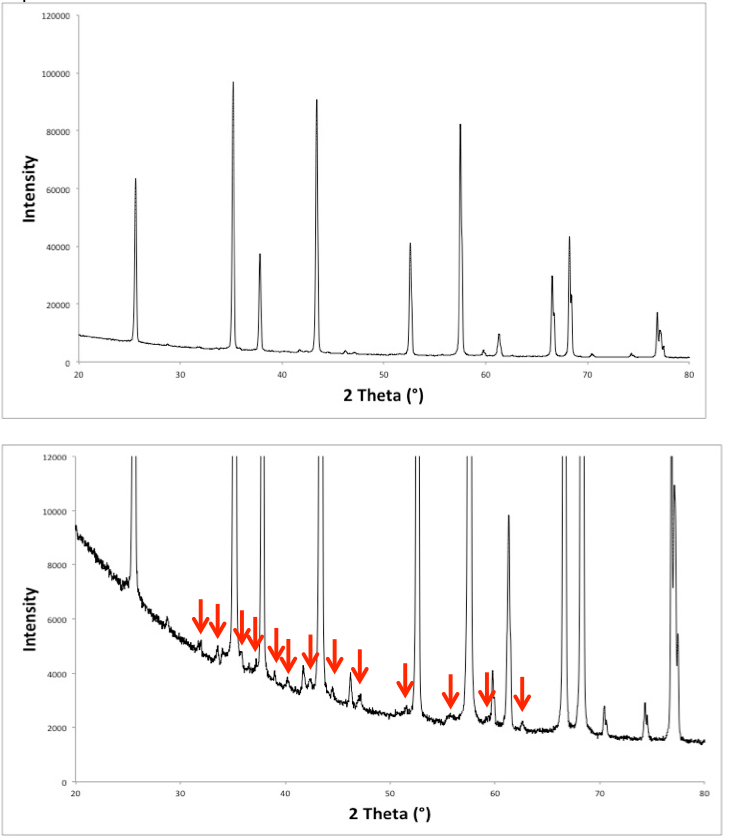
\includegraphics[width=\textwidth]{Chapter-5/Figures/Figure9.png}
	\caption{XRD pattern of a sample with 1060 ppm Na$_{2}$O, 82 ppm SiO$_{2}$, and 380 ppm MgO after sintering at 1525$^{\circ}$C for 5 h. The red arrows indicate the peaks that can be assigned to $\beta$-Al$_{2}$O$_{3}$. The other peaks can be assigned to $\alpha$-Al$_{2}$O$_{3}$.}
	\label{Ch5-figure:Figure9}
\end{figure}
%%%

\newpage
%%%
\begin{figure}[H]
	\centering
	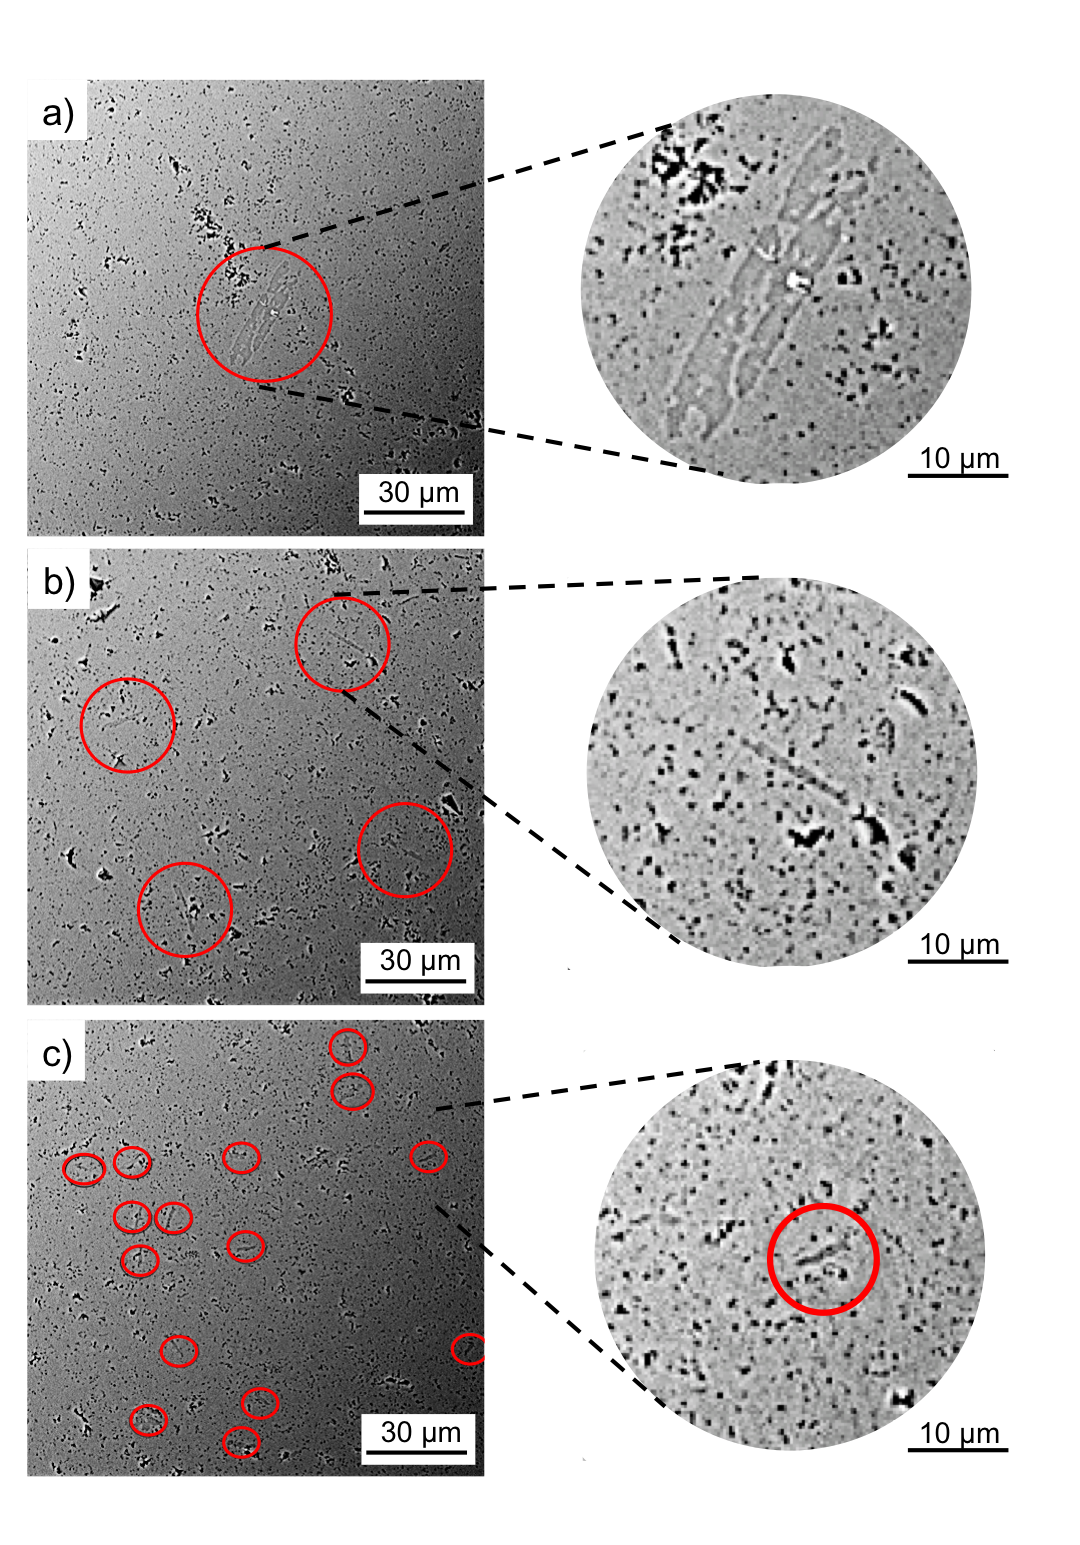
\includegraphics[width=\textwidth]{Chapter-5/Figures/Figure10.png}
	\caption{Micrograph showing $\beta$-Al$_{2}$O$_{3}$ grains (red circles) in an ultra high purity powder sample with 502 ppm Na$_{2}$O, 2 ppm MgO, and 11 ppm SiO$_{2}$ after sintering at 1525$^{\circ}$C for 0 h.}
	\label{Ch5-figure:Figure10}
\end{figure}
%%%

